\documentclass[11pt,letterpaper]{article}
\usepackage{amssymb,amsfonts,color,graphicx,amsmath,enumerate}
\usepackage{tikz}
\usepackage{amsthm}

\newcommand{\naturals}{\mathbb{N}}
\newcommand{\integers}{\mathbb{Z}}
\newcommand{\complex}{\mathbb{C}}
\newcommand{\reals}{\mathbb{R}}
\newcommand{\mcal}[1]{\mathcal{#1}}
\newcommand{\rationals}{\mathbb{Q}}
\newcommand{\Lp}[2]{\left\|{#1}\right\|_{L^{#2}}}
\newcommand{\F}{\mathbb{F}}
\newcommand{\affine}{\mathbb{A}}
\newcommand{\E}{\mathbb{E}}
\newcommand{\Prob}{\mathbb{P}}
\newcommand{\Var}{\text{Var}}
\newcommand{\ind}{\mathbbm{1}}
\newcommand{\Cov}{\text{Cov}}

\newenvironment{solution}
{\begin{proof}[Solution]}
{\end{proof}}

\voffset=-3cm
\hoffset=-2.25cm
\textheight=24cm
\textwidth=17.25cm
\addtolength{\jot}{8pt}
\linespread{1.3}

\begin{document}
\begin{center}
{\bf \Large Math 173A - Homework 4}
\vspace{0.2cm}
\hrule
\end{center}


% side channel attack on RSA
% probabilistic encryption
% RSA with CRT
% Fermat factorization

\begin{enumerate}

\item Do the following book exercises: 3.1(a) and (b), 3.8, 3.10 (you can use a computer or calculator), 3.11, 3.15(a), 3.22(a), 3.26(c).


\item Consider this variant of the square-and-multiply algorithm.
To compute $g^A\pmod N$, the algorithm scans the bits of $A$ from left (the most significant bit) to right (the least significant bit).
Set the initial result to $g$.
For every exponent bit, the current result is squared.
If and only if the currently scanned exponent bit is a 1, a multiplication of the current result by $g$ is executed after squaring.

\begin{enumerate}
    \item Use this algorithm to compute $2^{26}\pmod {29}$.

    \item Compare this algorithm to the square-and-multiply algorithm we discussed in class.
    Is this one faster?
    Does it require more or less storage?
\end{enumerate}



\item In this exercise we'll investigate a \emph{side-channel} attack on RSA.
This kind of attack doesn't exploit any of the mathematical weaknesses of RSA, but instead exploits how the protocol is actually implemented.

The figure below shows the power consumption of a microcontroller performing the square-and-multiply algorithm from exercise 2.
If the microcontroller computes a squaring or a multiplication, the power consumption increases.
Due to the small intervals in between the loops, every iteration can be identified.
Fuerthermore, for each round we can identify whether a single squaring (short duration) or a squaring followed by a multiplication (long duration) is being computed.

\begin{center}
    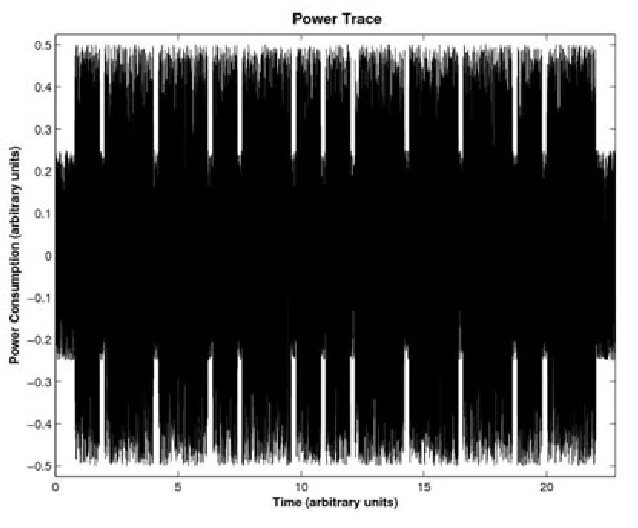
\includegraphics[scale=.45]{side channel.PNG}
\end{center}

\begin{enumerate}
    \item Identify the respective rounds in the figure and mark these with S for squaring or SM for squaring and multiplication (or just list them in order).

    \item Use the power consumption diagram to find the decryption exponent $d$.

    \item This key belongs to the RSA setup with the primes $p=67$ and $q=103$ and $e=257$.
    Verify your result form part (b). (Note that in practice an attacker wouldn't know the values of $p$ and $q$.)
\end{enumerate}

    

\end{enumerate}

\end{document}